\section{System Design}
\graphicspath{ {./images/} }

\subsection{Objectives}
\par The system design objectives are:
\begin{itemize}
	\item Establish the final expected result as idea/sketch 
	\item Sketch the functionality scheme for each module needed in detail.
	\item Setup a server with the necessary dependencies.
	\item Setup a database used for storing user records
	\item Site mockup for: home page, plugin page, calendar page, login page, register page, account page
	\item Implement basic interactions between user and platform: registration, login, CRUD (create-read-update-delete) for records, implement calendar feature, import Google Calendar, add plugins
	\item Implement Companion feature.
	\item Create the possibility to add user-made plugins 
	\item Live testing and deployment.
	
\end{itemize}


\subsection{Requirements specification}
\par Requirements to this platform are:  
\begin{enumerate}
	\item Intuitive and easy to use design  
	
	\item Assistant which will companion the user all the time  
	
	\item FAQ page  
	
	\item User Friendly 
	
	\item Adaptive web design 
	
	\item Deep personalization 
	
	\item Seamlessly API integration. 
	
	\item Community custom made plugins. 
\end{enumerate}



\subsection{UML Diagrams}
\subsubsection{Use case}
\par
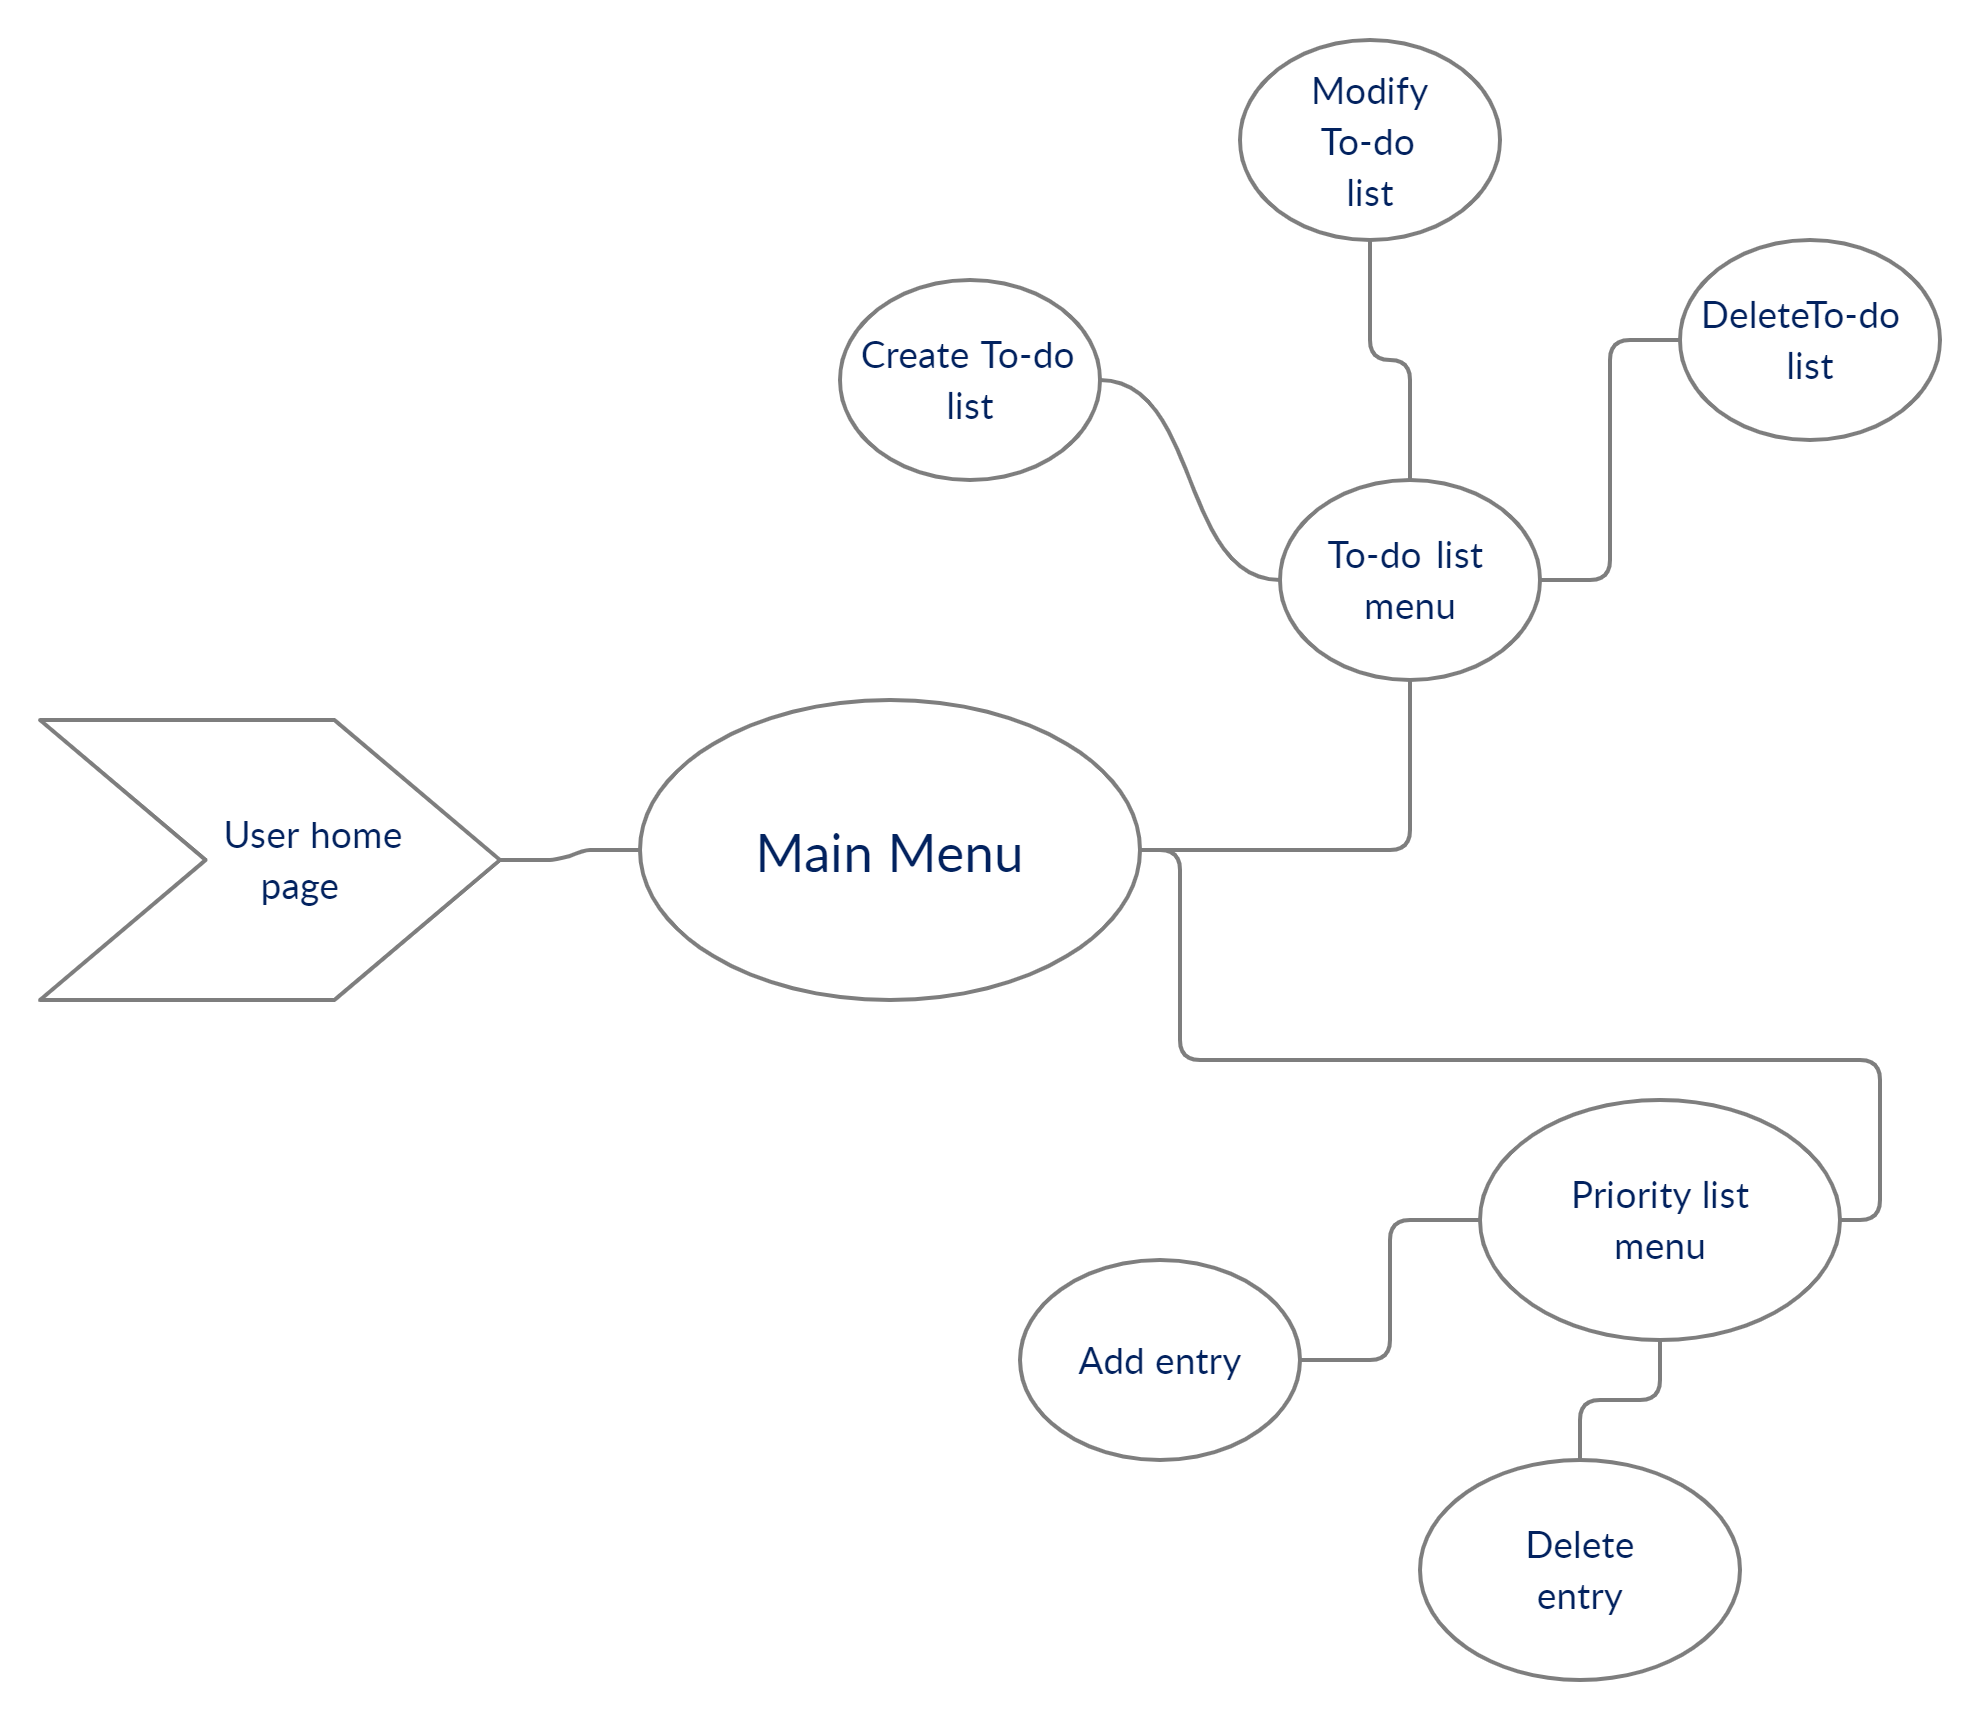
\includegraphics[width=\textwidth]{diagramusecase1}
\par
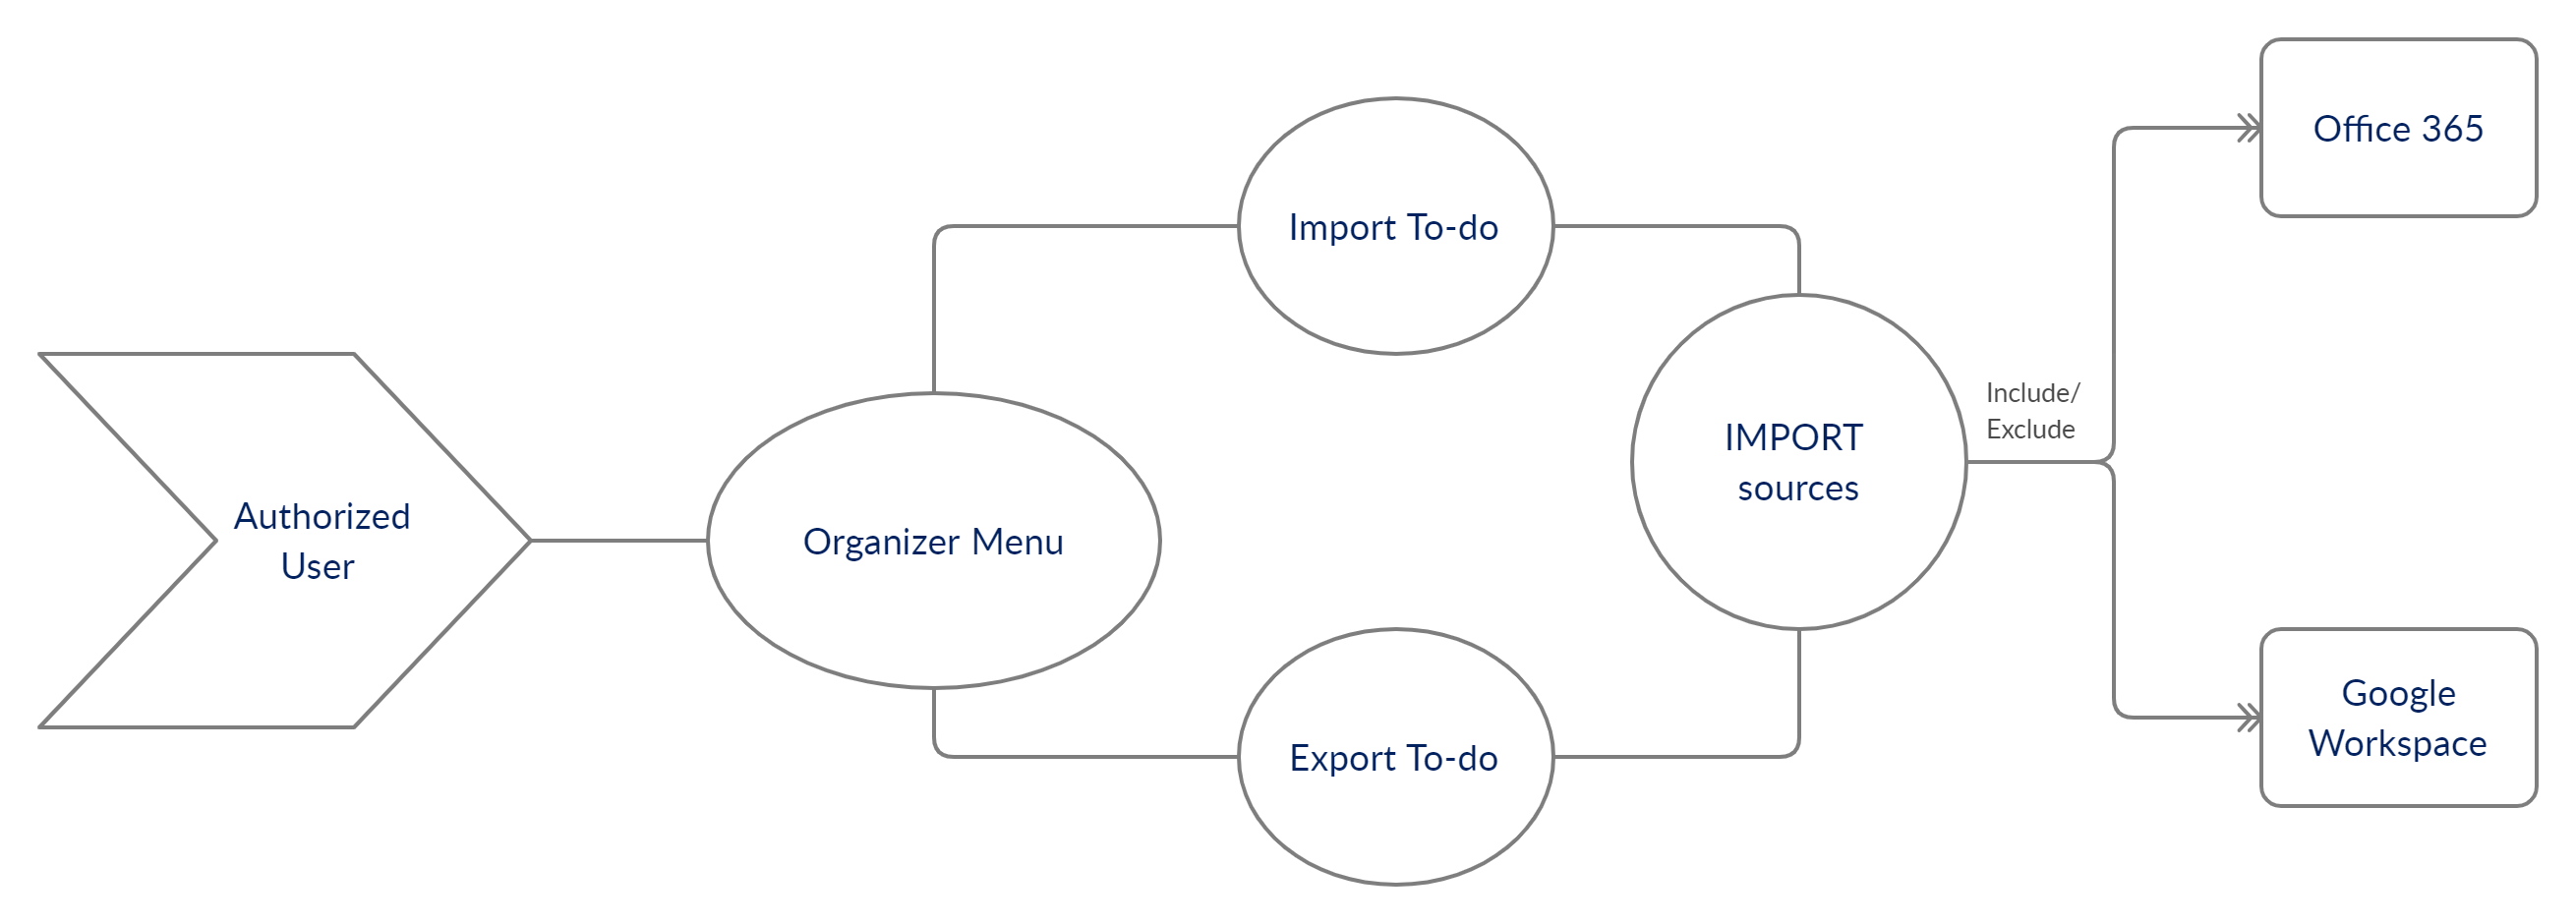
\includegraphics[width=\textwidth]{diagramusecase2}
\subsubsection{Component}
\par
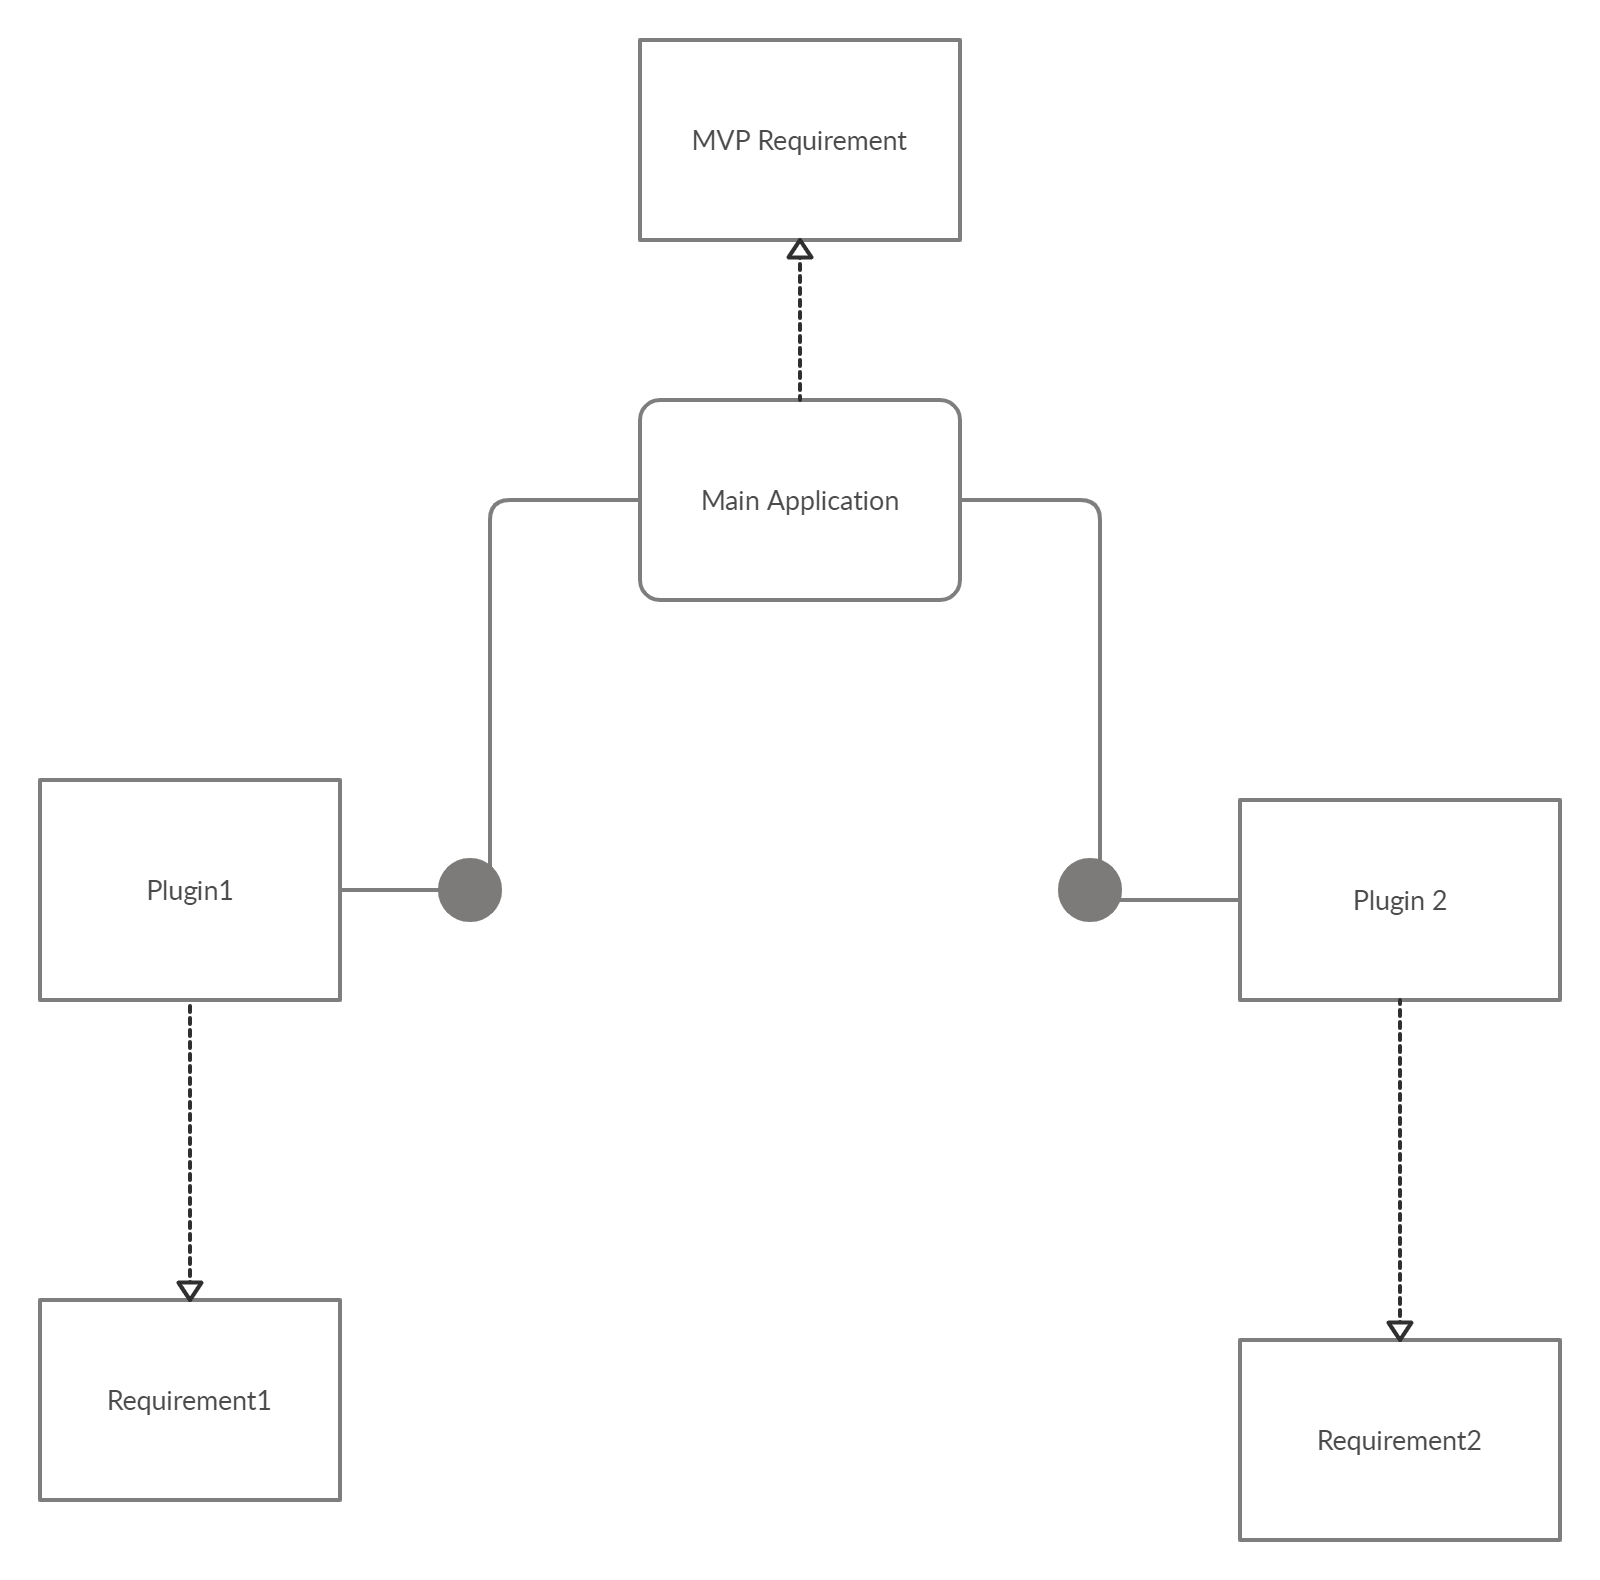
\includegraphics[width=\textwidth]{componentdigram1}
\subsection{Sequence}
\par
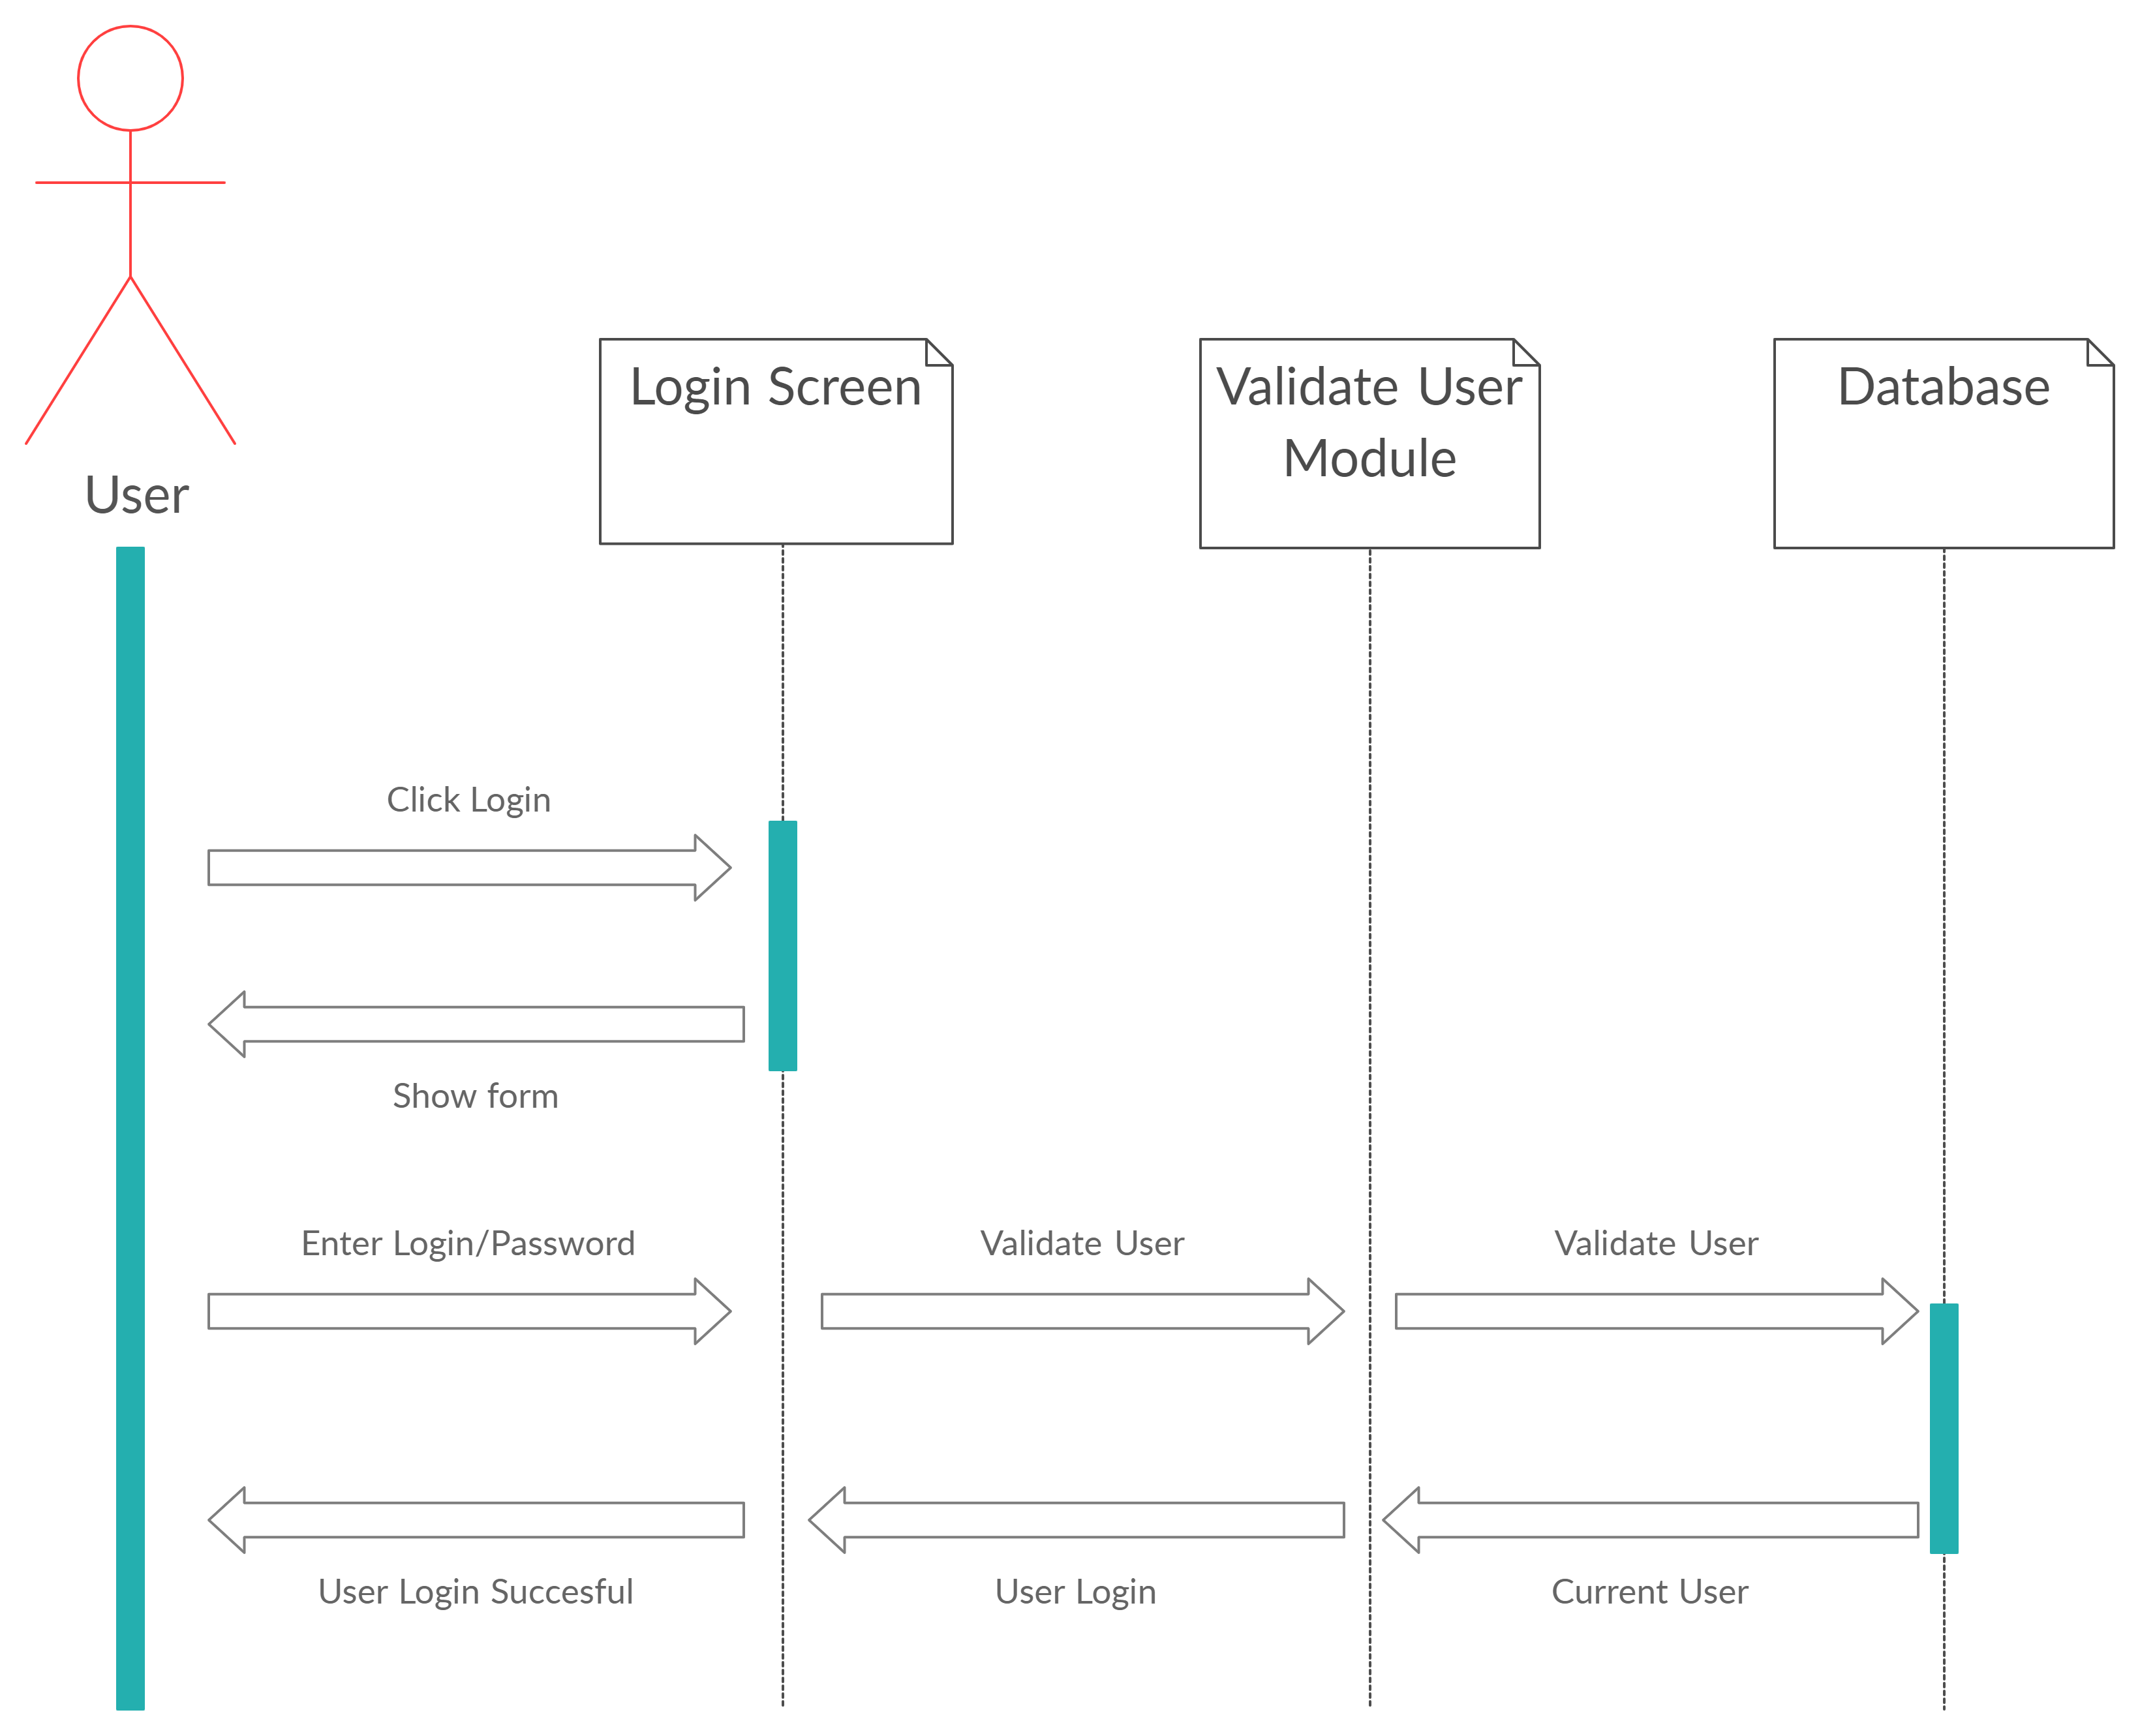
\includegraphics[width=\textwidth]{secuence digrram1}
\par
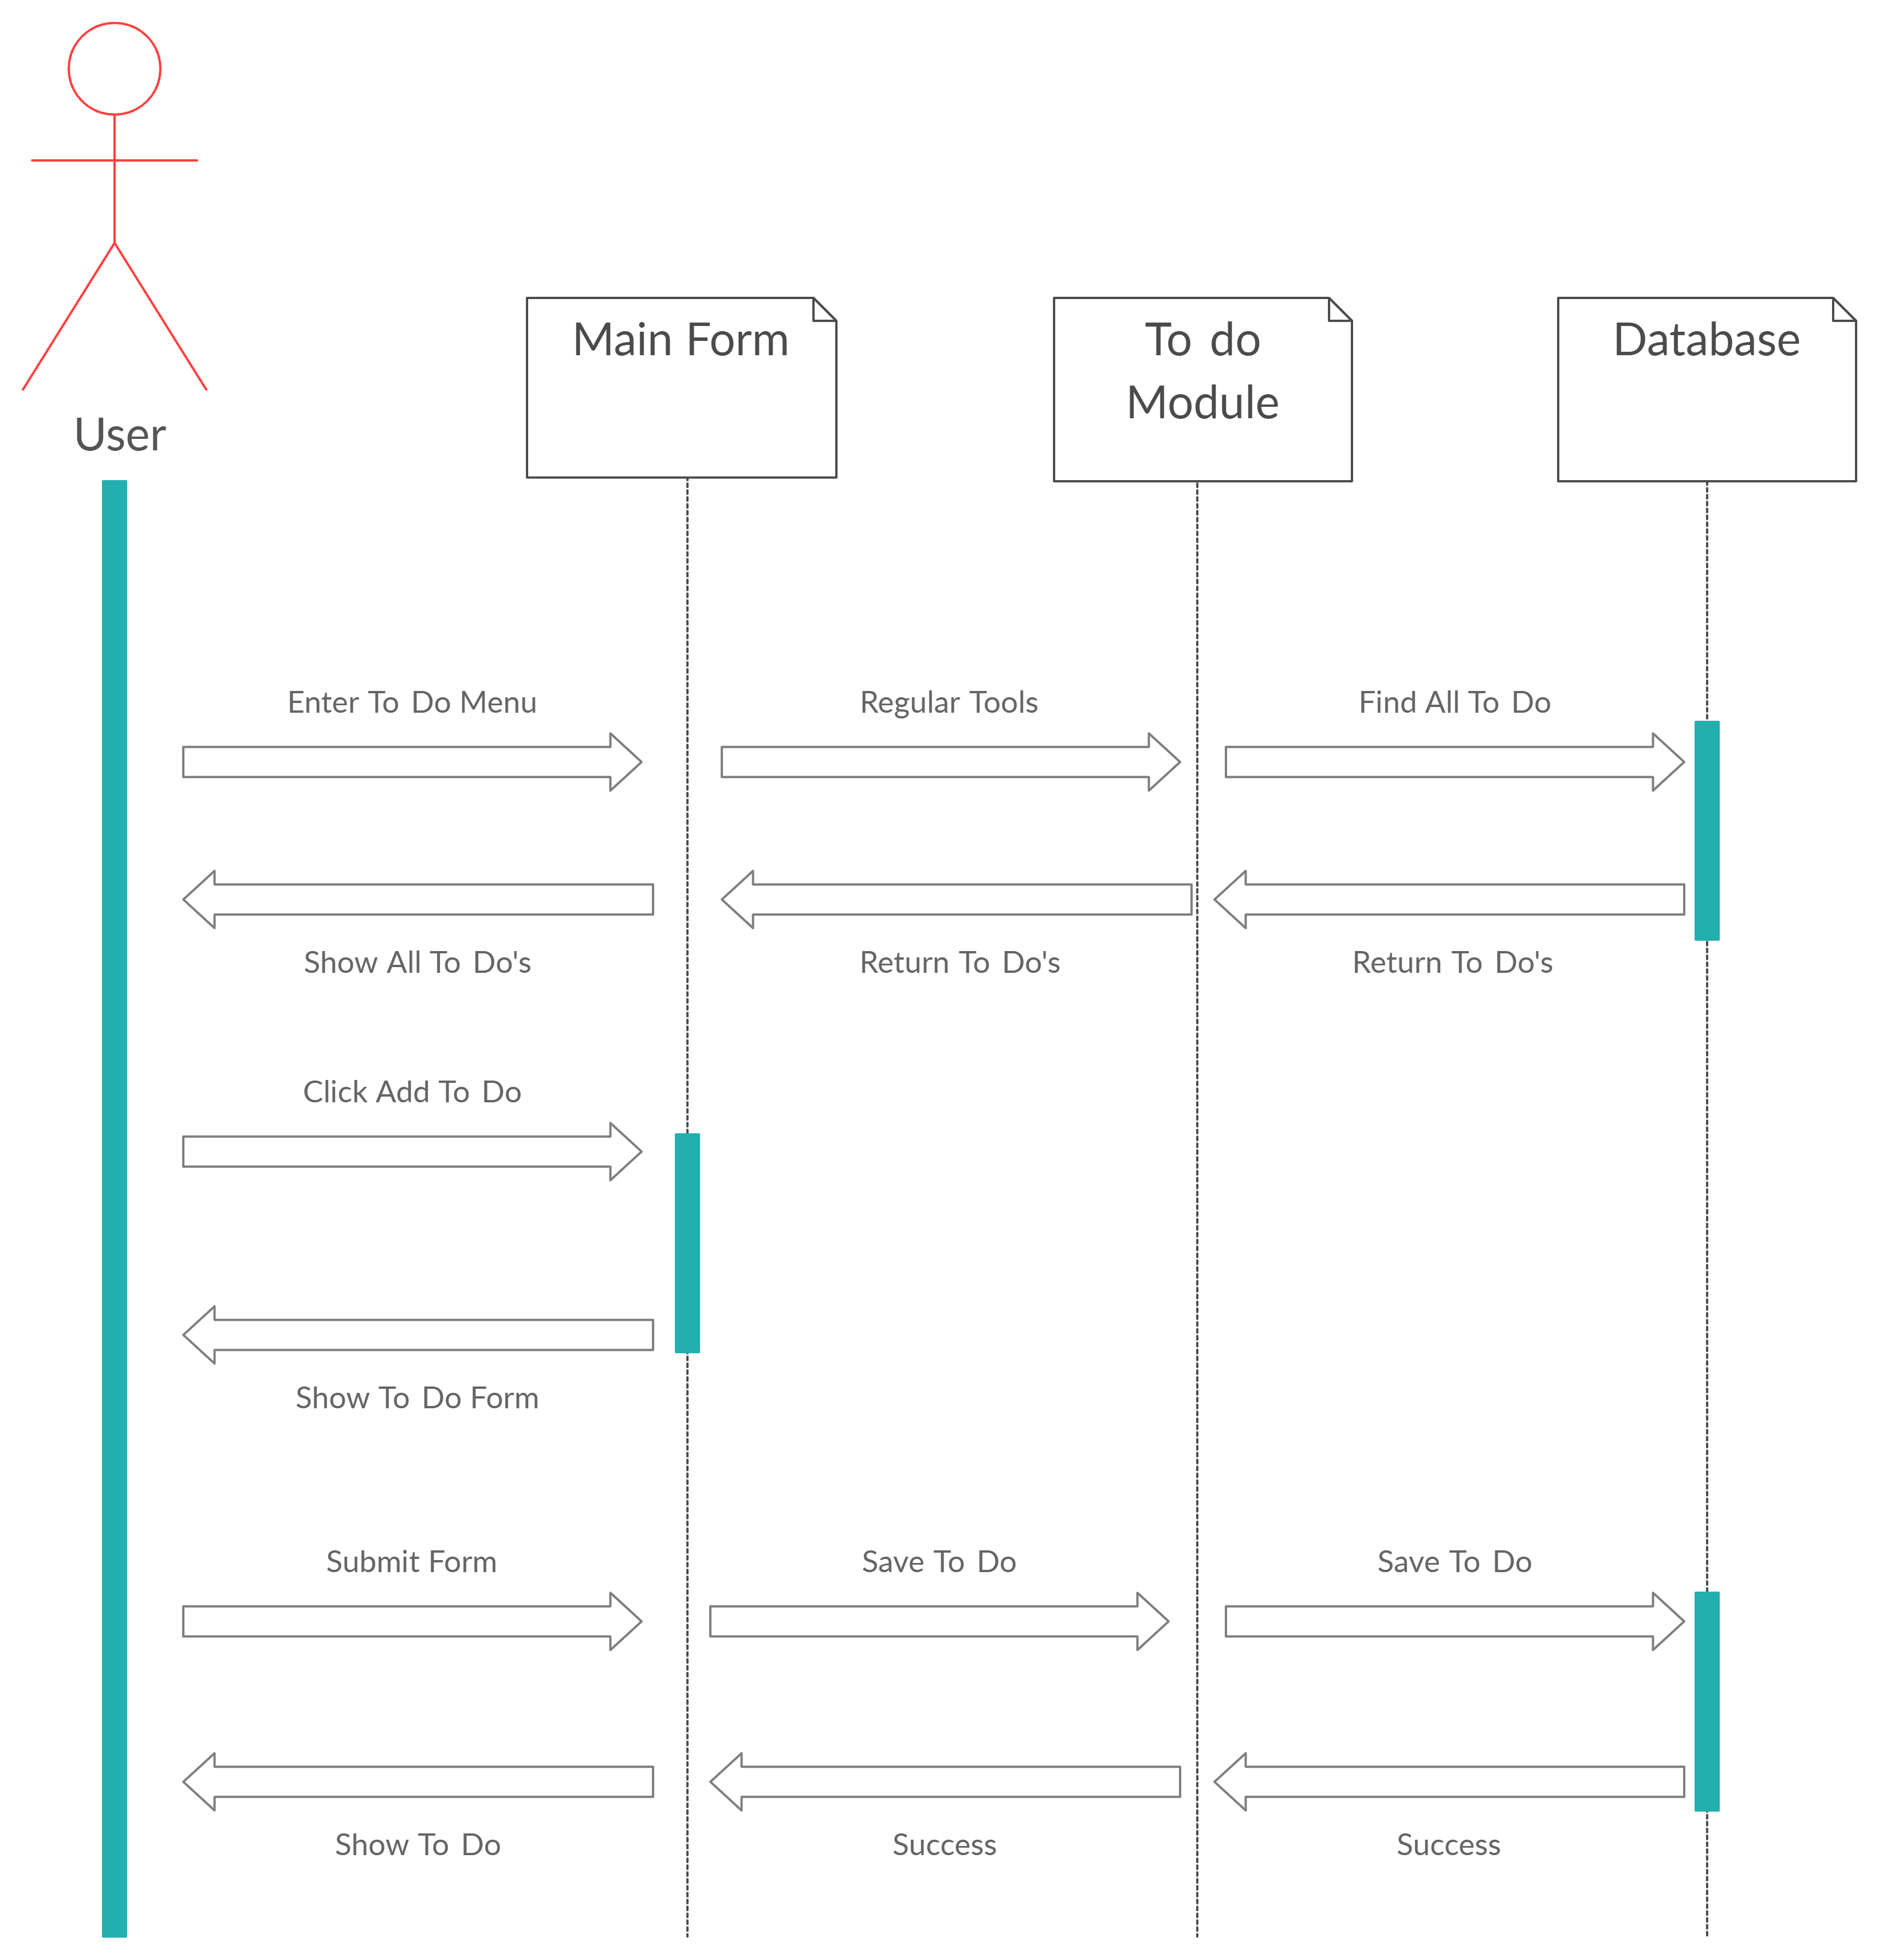
\includegraphics[width=\textwidth]{secuence digrram2}



\clearpage